\subsubsection{generation.roadgeneration}
    \textit{Roadgeneration} kapselt die Logik zur Generierung des eigentlichen Streckenverlaufs (\textit{Road}).\\
    Es bietet den anderen Generatoren Methoden zur Generierung unterschiedlicher Streckensegmente.\par

    \begin{figure}[htbp]
        \centering
        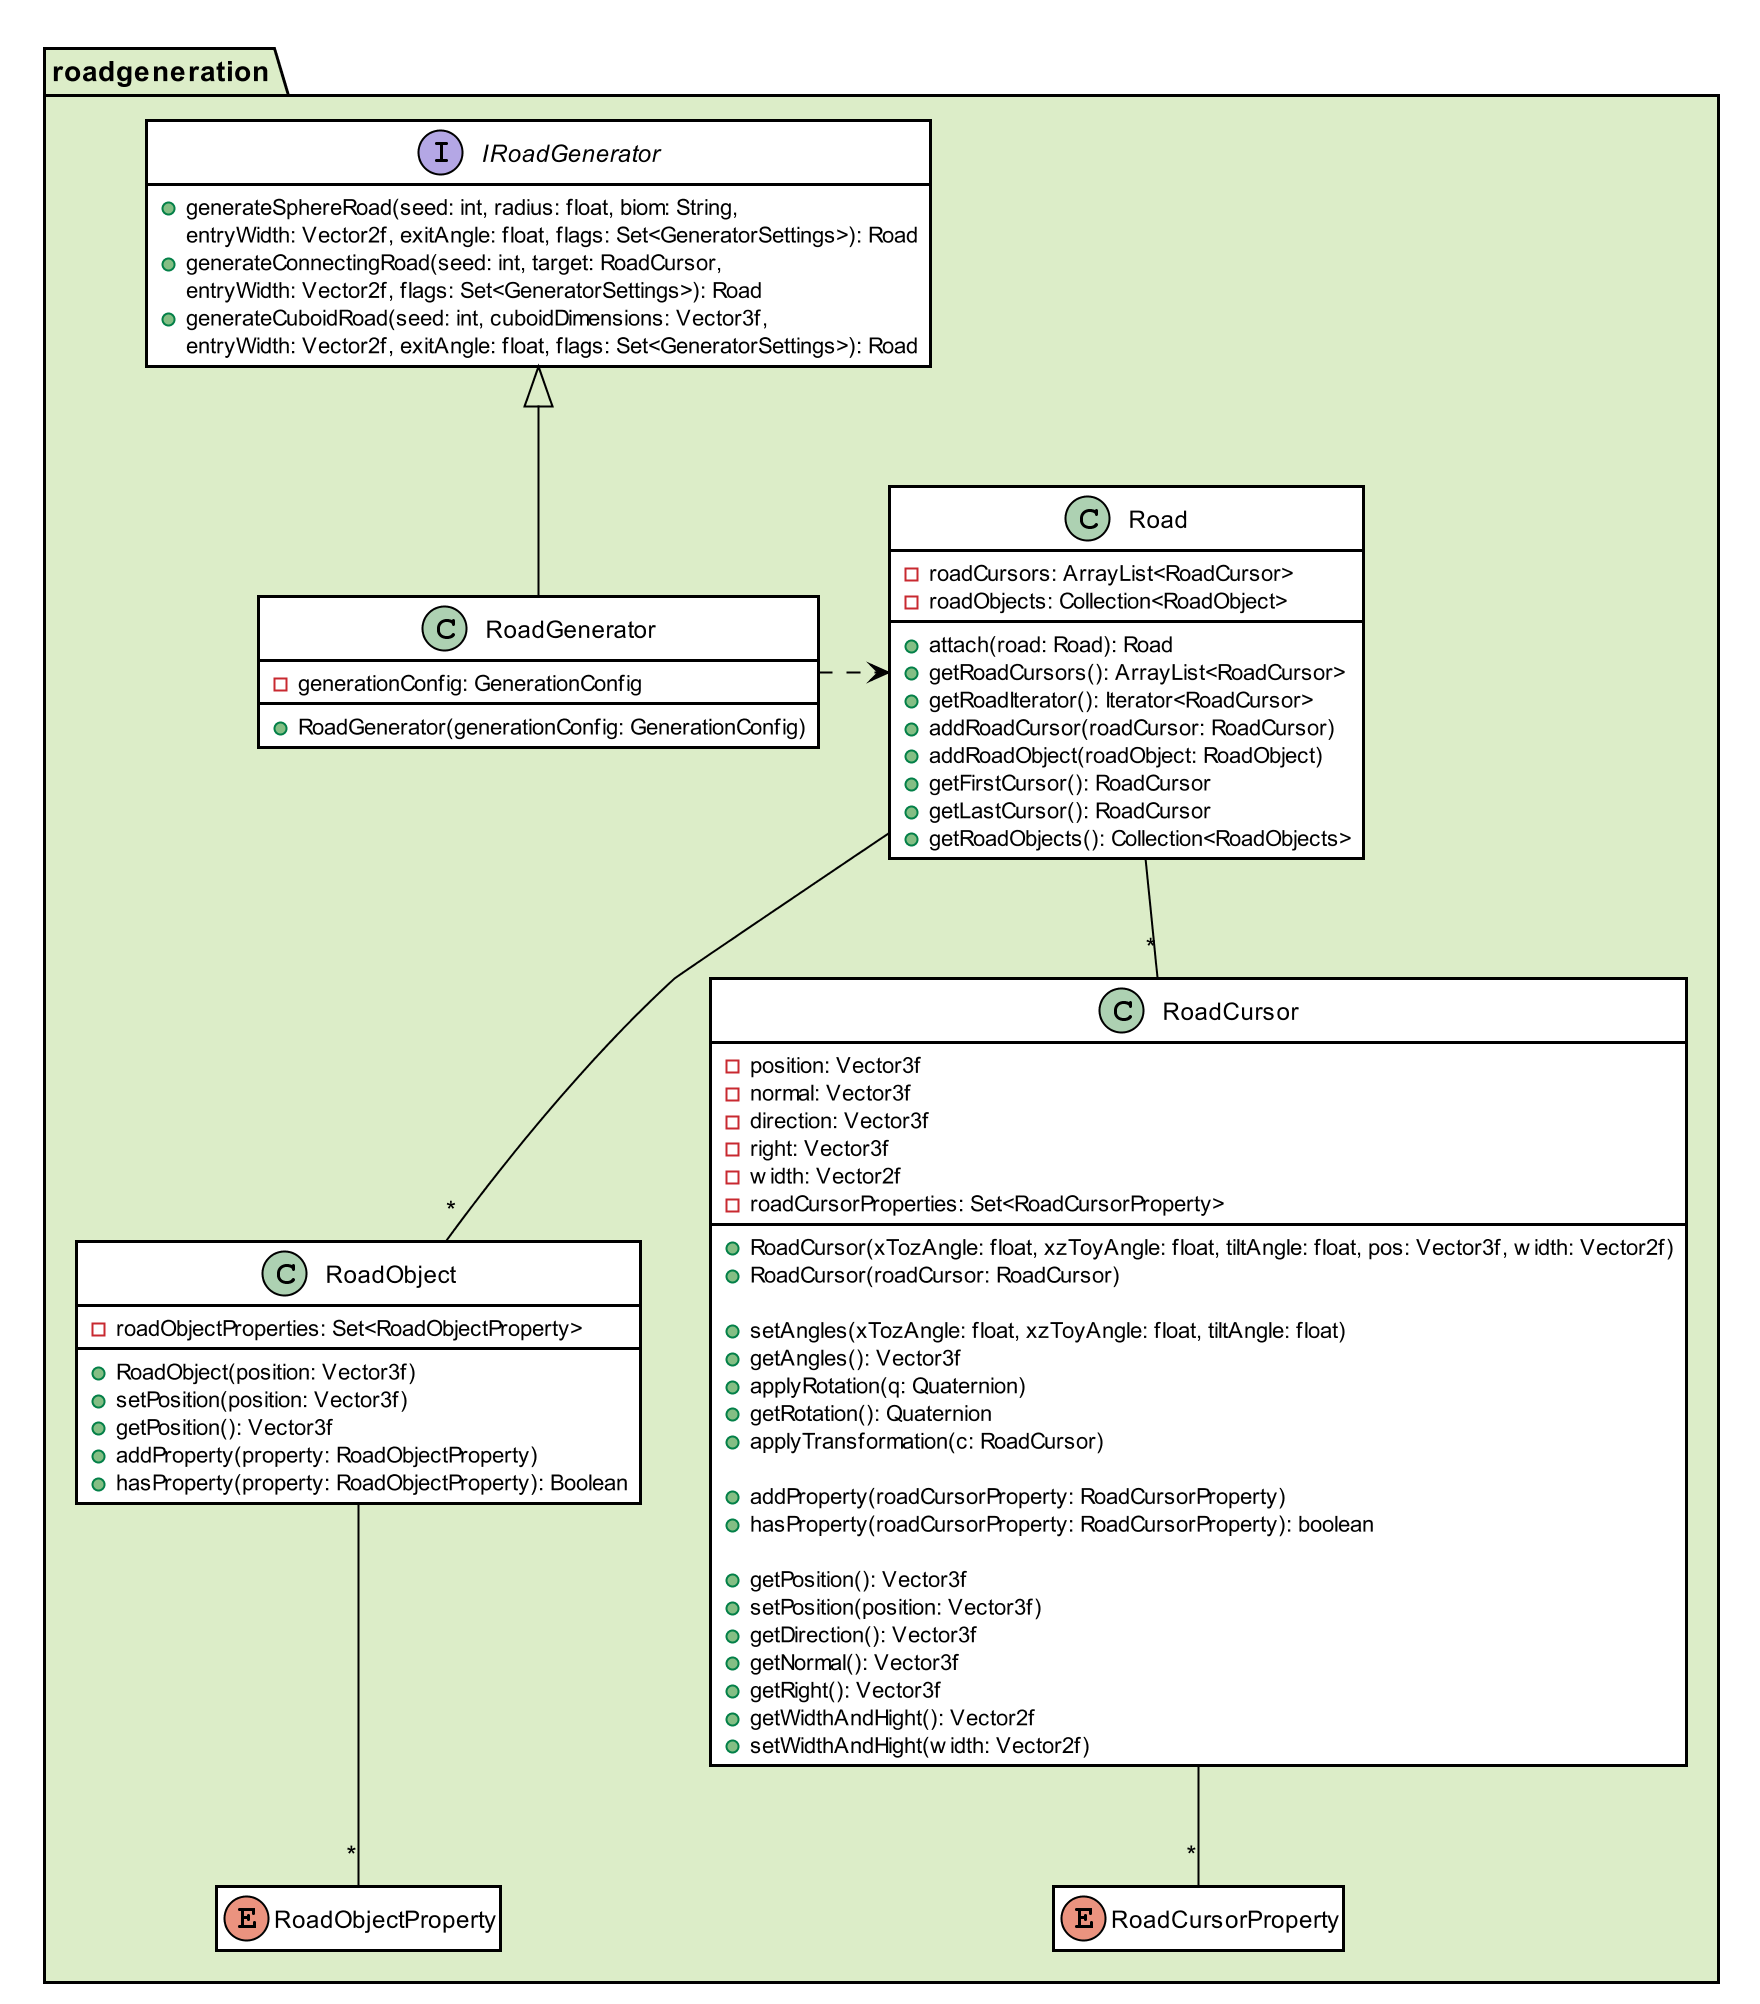
\includegraphics[width=0.9\linewidth]{./Generierung/Bilder/roadgeneration.png}
        \caption{Klassendiagramm domegeneration}
    \end{figure}

        \pagebreak
        \paragraph{\underline{IRoadGenerator}} \mbox{}\par
            Schnittstelle zur Generierung eines Streckenabschnitts.
            Ein ausgegebener Streckenabschnitt begint immer am Startpunkt (0,0,0) und Verläuft am Start in Z-Richtung.
            \par
            
            \textbf{Methoden}
            \begin{itemize}
                \item  \textit{+ generateSphereRoad(int seed, float radius, String biom,
                Vector2f entryWidth, float exitAngle, Collection<GeneratorSettings> flags): Road}
                    \begin{leftbar}[0.9\linewidth]
                        Erzeugt eine Strecke in einer Halbkugel, gegeben durch den Radius (\textit{radius}).\\
                        Die Strecke beginnt am Rande der Halbkugel.\\
                        Danach nimmt sie einen scheinbar belibigen Verlauf innerhalb der Halbkugel an.
                        Die Ausprägung des Verlaufs hängt vom Biom (\textit{biom}) ab.\\
                        Die Strecke terminiert wieder am Rande der Halbkugel.\\
                        Die Strecke kollidiert nie mit sich selber.\\
                        \textbf{@param seed} Zum bestimmen von Pseuozufallswerten, die den Verlauf der Strecke bestimmen.\\
                        \textbf{@param radius} Radius der Halbkugel.\\
                        \textbf{@param biom} Bestimmt Ausprägung der Stecke.\\
                        \textbf{@param entryWidth} Bestimmt den Querschnitt der Strecke am Eingang.\\
                        \textbf{@param exitAngle} Zahl zwischen [-Pi,PI]. Präferierter Winkel zwischen Ein- und Ausgang.\\
                        \textbf{@param Collection<GeneratorSettings> flags} Kollektion an Parametern, die als Präferenzen zur Generierung dienen.\\
                        \textbf{@return} Datenstruktur (\textit{Road}), die eine Strecke beschreibt.
                    \end{leftbar}

                \item  \textit{+ generateConnectingRoad(int seed, RoadCursor target,
                Vector2f entryWidth, Collection<GeneratorSettings> flags): Road}
                    \begin{leftbar}[0.9\linewidth]
                        Erzeugt eine Verbindungsstrecke vom Startpunkt zum relativen Zielpunkt (\textit{RoadCursor target}).\\
                        \textbf{@param seed} Zum bestimmen von Pseuozufallswerten, die den Verlauf der Strecke beeinflussen.\\
                        \textbf{@param target} Beschreibt den Zielpunkt der Strecke aus dem Bezugssystem des Eingangspunkt\\
                        \textbf{@param entryWidth} Bestimmt den Querschnitt der Strecke am Eingang.\\
                        \textbf{@param Collection<GeneratorSettings> flags} Kollektion an Parametern, die als Präferenzen zur Generierung dienen.\\
                        \textbf{@return} Datenstruktur (\textit{Road}), die eine Strecke beschreibt.
                    \end{leftbar}

                \pagebreak

                \item  \textit{+ generateCuboidRoad(int seed, Vector3f cuboidDimensions,
                Vector2f entryWidth, float exitAngle, Collection<GeneratorSettings> flags): Road}
                    \begin{leftbar}[0.9\linewidth]
                        Erzeugt eine Strecke durch einen Quader, beschrieben durch \textit{cuboidDimensions}.
                        Ausgang und Eingang befinden sich rechtwinklig zu den jeweiligen Wänden des Quaders, an denen sie platziert sind.\\
                        \textbf{@param seed} Zum bestimmen von Pseuozufallswerten, die den Verlauf der Strecke beeinflussen.\\
                        \textbf{@param cuboidDimensions} Dimension des Quaders\\
                        \textbf{@param entryWidth} Bestimmt den Querschnitt der Strecke am Eingang.\\
                        \textbf{@param exitAngle} Zahl zwischen [-Pi,PI]. Präferierter Winkel zwischen Ein- und Ausgang.\\
                        \textbf{@param Collection<GeneratorSettings> flags} Kollektion an Parametern, die als Präferenzen zur Generierung dienen.\\
                        \textbf{@return} Datenstruktur (\textit{Road}), die eine Strecke beschreibt.
                    \end{leftbar}
            \end{itemize}


        \paragraph{\underline{RoadGenerator}} \mbox{}\par
            Implementierung der Schnittstelle (\textit{IRoadGenerator}) zur Generierung eines Streckenabschnitts.
            \par

            \textbf{Atribute}					
            \begin{itemize}
                \item  \textit{GenerationConfig generationConfig}
                    \begin{leftbar}[0.9\linewidth]
                        Datenstruktur, die Parameter für die Generierung hält.\\
                    \end{leftbar}
            \end{itemize}
            \textbf{Methoden}					
            \begin{itemize}
                \item  \textit{+ RoadGenerator(GenerationConfig generationConfig)}
                    \begin{leftbar}[0.9\linewidth]
                        Erzeugt einen neuen \textit{RoadGenerator}.
                        \textbf{@param generationConfig} Datenstruktur, die Parameter für die Generierung hält.\\
                    \end{leftbar}
            \end{itemize}



        \paragraph{\underline{Road}} \mbox{}\par
            Datenstruktur zur Darstellung der Strecke.
            \par



            \textbf{Atribute}					
            \begin{itemize}
                \item  \textit{ArrayList<RoadCursor> roadCursors}
                    \begin{leftbar}[0.9\linewidth]
                        List an \textit{RoadCursor} welche den Verlauf der \textit{Road} bestimmen.\\
                    \end{leftbar}
                \item  \textit{Collection<RoadObject> roadObjects}
                \begin{leftbar}[0.9\linewidth]
                    Menge an \textit{RoadObjects} welche auf der \textit{Road} positionierte Objekte (zB Items) darstellen.\\
                \end{leftbar}
            \end{itemize}


        
            \textbf{Methoden}					
            \begin{itemize}
                \item  \textit{+ attach(Road road): Road }
                    \begin{leftbar}[0.9\linewidth]
                        Hängt die gegebene \textit{road} ans Ende dieser Strecke an.\\
                        Die Position und Orientierung aller in der \textit{road} enthaltenen \textit{RoadCursor},
                        wird ins Bezugsystem des ersten \textit{RoadCursor} dieser Strecke umgerechnet.\\
                        \textbf{@param road} Die Strecke welche an diese Strecke angehängt wird.\\
                    \end{leftbar}
            
                \item  \textit{+ getRoadCursors(): ArrayList<RoadCursor>}
                    \begin{leftbar}[0.9\linewidth]
                        Gibt eine Liste aller \textit{RoadCursor} in ihrer Reihenfolge aus.\\
                        \textbf{@return} Liste aller \textit{RoadCursor} in ihrer Reihenfolge.\\
                    \end{leftbar}
            
                \item  \textit{+ getRoadCursorIterator(): Iterator<RoadCursor>}
                    \begin{leftbar}[0.9\linewidth]
                        Gibt einen Iterator über die Liste aller \textit{RoadCursor} in ihrer Reihenfolge aus.\\
                        \textbf{@return} Iterator über die Liste aller \textit{RoadCursor} in ihrer Reihenfolge.\\
                    \end{leftbar}
            
                \item  \textit{+ addRoadCursor(RoadCursor roadCursor)}
                    \begin{leftbar}[0.9\linewidth]
                        Fügt einen weiteren RoadCursor ans Ende der \textit{Road} an.\\
                        \textbf{@return} \textit{RoadCursor} welcher der \textit{Road} angefügt werden soll.\\
                    \end{leftbar}

                \item  \textit{+ addRoadObject(RoadObject roadObject)}
                    \begin{leftbar}[0.9\linewidth]
                        Fügt der \textit{Road} ein \textit{RoadObject} hinzu.\\
                        \textbf{@return} \textit{RoadObject} welcher der \textit{Road} hinzugefügt werden soll.\\
                    \end{leftbar}
            
                \item  \textit{+ getFirstRoadCursor(): RoadCursor}
                    \begin{leftbar}[0.9\linewidth]
                        Gibt den ersten \textit{RoadCursor} der \textit{Road} zurück.\\
                        \textbf{@return} Erster \textit{RoadCursor} der \textit{Road}.\\
                    \end{leftbar}
            
                \item  \textit{+ getLastRoadCursor(): RoadCursor}
                    \begin{leftbar}[0.9\linewidth]
                        Gibt den letzten \textit{RoadCursor} der \textit{Road} zurück.\\
                        \textbf{@return} Letzter \textit{RoadCursor} der \textit{Road}.\\
                    \end{leftbar}
            
                \item  \textit{+ getRoadObjects(): Collection<RoadObjects>}
                    \begin{leftbar}[0.9\linewidth]
                        Gibt die Menge aller \textit{RoadObjects} aus, welche die \textit{Road} enthält.\\
                        \textbf{@return} Menge aller \textit{RoadObjects} der \textit{Road}.\\
                    \end{leftbar}
            
                \item  \textit{+ addRoadObject(RoadObjects roadObject)}
                    \begin{leftbar}[0.9\linewidth]
                        Fügt der \textit{roadObject} der \textit{Road} hinzu.\\
                        \textbf{@return} \textit{RoadCursor} welcher der \textit{Road} hinzugefügt wird.\\
                    \end{leftbar}
            \end{itemize}

        \paragraph{\underline{RoadCursor}} \mbox{}\par
            Datenstruktur zur Darstellung eines Streckenpunktes im dreidimensionalen Raum.\\
            Dieser ist repräsentiert durch eine Position und einem Koordinatensystem mit 3 Achsen.\\
            Des weiteren enthält er die Breite und Höhe der Strecke in diesem Punkt und eine Menge an Eigenschaften.
            Der RoadCursor markiert immer die Mitte der Straße.
            \par

            \textbf{Atribute}
            \begin{itemize}

                \item  \textit{Vector3f position}
                    \begin{leftbar}[0.9\linewidth]
                        Position des \textit{RoadCursor}
                    \end{leftbar}
                
                \item  \textit{Vector3f normal}
                    \begin{leftbar}[0.9\linewidth]
                        Y-Achse des durch \textit{RoadCursor} repräsentierten Koordinaten \textit{RoadCursor}\\
                        Normalenvektor zur Strecke in diesem Punkt.
                    \end{leftbar}

                \item  \textit{Vector3f direction}
                    \begin{leftbar}[0.9\linewidth]
                        Z-Achse des durch \textit{RoadCursor} repräsentierten Koordinaten \textit{RoadCursor}\\
                        Richtungsvektor der Strecke in diesem Punkt.
                    \end{leftbar}

                \item  \textit{Vector3f right}
                    \begin{leftbar}[0.9\linewidth]
                        X-Achse des durch \textit{RoadCursor} repräsentierten Koordinaten \textit{RoadCursor}\\
                        Rechtsvektor der Strecke in diesem Punkt.
                    \end{leftbar}
                
                \item  \textit{Vector2f widhtAndHight}
                    \begin{leftbar}[0.9\linewidth]
                        Breite und Höhe und Höhe der Strecke in diesem Punkt.
                    \end{leftbar}
                \item  \textit{Set<RoadCursorProperty> roadCursorProperties}
                    \begin{leftbar}[0.9\linewidth]
                        Eigenschaften des \textit{RoadCursor} (zB. Checkpoint)
                    \end{leftbar}
            

            \end{itemize}

        \textbf{Methoden}
        \begin{itemize}

            \item  \textit{+ RoadCursor(float xTozAngle, float xzToyAngle, float tiltAngle, Vector3f position, Vector2f width)}
                \begin{leftbar}[0.9\linewidth]
                    Erstellt einen neuen \textit{RoadCursor} anhand gegebener Parameter.\\
                    \textbf{@param xTozAngle} Rotationswinkel um die Y-Achse.\\
                    \textbf{@param xzToyAngle} Steigungswinkel.\\
                    \textbf{@param tiltAngle} Seitliche Neigung der Strecke.\\
                    \textbf{@param position} Positionsvektor.\\
                    \textbf{@param width} Breite und Höhe der Strecke.\\
                \end{leftbar}

            \item  \textit{+ RoadCursor(RoadCursor roadCursor)}
                \begin{leftbar}[0.9\linewidth]
                    Erstellt einen neuen \textit{RoadCursor} der eine echte Kopie des gegebenen \textit{RoadCursors} ist.\\
                    \textbf{@param roadCursor} \textit{RoadCursor} der kopiert werden soll.
                \end{leftbar}

            \pagebreak

            \item  \textit{+ setAngles(float xTozAngle, float xzToyAngle, float tiltAngle)}
                \begin{leftbar}[0.9\linewidth]
                    Bestimmt die Ausrichtung des \textit{RoadCursors} durch 3 Winkel.\\
                    \textbf{@param xTozAngle} Rotationswinkel um die Y-Achse.\\
                    \textbf{@param xzToyAngle} Steigungswinkel.\\
                    \textbf{@param tiltAngle} Seitliche Neigung der Strecke.
                \end{leftbar}
                    

            \item  \textit{+ getAngles(): Vector3f}
                \begin{leftbar}[0.9\linewidth]
                    Gibt die Ausrichtung des \textit{RoadCursors} durch 3 Winkel zurück.\\
                    \textbf{@return} (Rotationswinkel um die Y-Achse, Steigungswinkel, Seitliche Neigung der Strecke).
                \end{leftbar}

            \item  \textit{+ applyRotation(Quaternion q)}
                \begin{leftbar}[0.9\linewidth]
                    Wendet die durch den gegebenen \textit{Quaternion} definierte Rotation auf alle Achsen des Koordinatensystems an.\\
                    \textbf{@param} \textit{Quaternion} welcher von der jMonkeyEngine zur Darstellung von Rotationen verwendet wird.
                \end{leftbar}

            \item  \textit{+ getRotation(): Quaternion}
                \begin{leftbar}[0.9\linewidth]
                    Gibt die Ausrichtung des \textit{RoadCursors} als \textit{Quaternion} zurück.\\
                    \textbf{@return} \textit{Quaternion} welcher von der jMonkeyEngine zur Darstellung von Rotationen verwendet wird.
                \end{leftbar}

            \item  \textit{+ applyTransformation(RoadCursor c)}
                \begin{leftbar}[0.9\linewidth]
                    Transformiert die aktuelle Position um die durch \textit{c} gegebene Position\\
                    und rotiert diesen \textit{RoadCursors} um die durch c gegebene Rotation \\
                    \textbf{@param c} \textit{RoadCursors} welcher die Transformation definiert
                \end{leftbar}

            \item  \textit{+ addProperty(RoadCursorProperty roadCursorProperty)}
                \begin{leftbar}[0.9\linewidth]
                    Fügt diesem \textit{RoadCursors} eine \textit{RoadCursorProperty} hinzu.\\
                    \textbf{@param roadCursorProperty} \textit{RoadCursorProperty} welche hinzugefügt werden soll
                \end{leftbar}
            
            \item  \textit{+ hasProperty(RoadCursorProperty roadCursorProperty): boolean}
                \begin{leftbar}[0.9\linewidth]
                    Gibt aus ob der \textit{RoadCursors} die gegebene \textit{RoadCursorProperty} enthält.\\
                    \textbf{@param roadCursorProperty} \textit{RoadCursorProperty} auf welche geprüft werden soll\\
                    \textbf{@return} Wahr, falls der \textit{RoadCursors} die gegebene \textit{RoadCursorProperty} enthält. Sonst falsch.
                \end{leftbar}

            \item  \textit{+ getPosition(): Vector3f}
                \begin{leftbar}[0.9\linewidth]
                    Gibt die Position des \textit{RoadCursors} zurück.\\
                    \textbf{@return} Position des \textit{RoadCursors}.
                \end{leftbar}

            \item  \textit{+ setPosition(Vector3f position)}
                \begin{leftbar}[0.9\linewidth]
                    Setzt die Position des \textit{RoadCursors}.\\
                    \textbf{@param} Positionsvektor.
                \end{leftbar}

            \pagebreak
            
            \item  \textit{+ getDirection(): Vector3f}
                \begin{leftbar}[0.9\linewidth]
                    Gibt den Richtungsvektor des \textit{RoadCursors} zurück.\\
                    \textbf{@return} Richtungsvektor.
                \end{leftbar}


            \item  \textit{+ getNormal(): Vector3f}
                \begin{leftbar}[0.9\linewidth]
                    Gibt den Normalenvektor des \textit{RoadCursors} zurück.\\
                    \textbf{@return} Normalenvektor.
                \end{leftbar}

            \item  \textit{+ getRight(): Vector3f}
                \begin{leftbar}[0.9\linewidth]
                    Gibt den Rechtsvektor des \textit{RoadCursors} zurück.\\
                    \textbf{@return} Rechtsvektor.
                \end{leftbar}

            \item  \textit{+ getWidhtAndHight(): Vector3f}
                \begin{leftbar}[0.9\linewidth]
                    Gibt die Breite und Höhe des \textit{RoadCursors} zurück.\\
                    \textbf{@return} Breite.
                \end{leftbar}

            \item  \textit{+ setWidhtAndHight(Vector2f width): Vector3f}
                \begin{leftbar}[0.9\linewidth]
                    Setzt die Breite und Höhe des \textit{RoadCursors}.\\
                    \textbf{@param} Breite.
                \end{leftbar}
        \end{itemize}

    \paragraph{\underline{RoadCursorProperty}} \mbox{}\par
    Eigenschaft zur Charakterisierung eines \textit{RoadCursors}
    (zB. zur Darstellung eines Checkpoints).
    \par

    \pagebreak
    \paragraph{\underline{RoadObject}} \mbox{}\par
        Auf der Strecke plazierbares Objekt
        (zB. zur Darstellung von Items, Startpositionen).
        \par

        \textbf{Atribute}
            \begin{itemize}

                \item  \textit{Set<RoadObjectProperty> roadObjectProperty}
                    \begin{leftbar}[0.9\linewidth]
                        Eigenschaften welche den Typ des \textit{RoadObject} bestimmen.\\
                    \end{leftbar}

            \end{itemize}
        
        \textbf{Methoden}
        \begin{itemize}

            \item  \textit{+ RoadObject(Vector3f position)}
                \begin{leftbar}[0.9\linewidth]
                    Erstellt ein neues \textit{RoadObject} anhand an einer Position.\\
                    \textbf{@param position} Positionsvektor.
                \end{leftbar}

            \item  \textit{+ setPosition(Vector3f position)}
                \begin{leftbar}[0.9\linewidth]
                    Setzt die Position.\\
                    \textbf{@param position} Positionsvektor.
                \end{leftbar}
            
            \item  \textit{+ getPosition(): Vector3f}
                \begin{leftbar}[0.9\linewidth]
                    Gibt die Position zurück.\\
                    \textbf{@param position} Positionsvektor.
                \end{leftbar}

            \item  \textit{+ addProperty(RoadObjectProperty property)}
                \begin{leftbar}[0.9\linewidth]
                    Fügt dem \textit{RoadObject} eine \textit{RoadObjectProperty} hinzu.\\
                    \textbf{@param property} \textit{RoadObjectProperty}.
                \end{leftbar}
            
            \item  \textit{+ hasProperty(RoadObjectProperty property): Boolean}
                \begin{leftbar}[0.9\linewidth]
                    Gibt aus ob das \textit{RoadObject} die gegebene \textit{RoadObjectProperty} enthält.\\
                    \textbf{@param property} Wahr, falls das \textit{RoadObject} die gegebene \textit{RoadObjectProperty} enthält. Sonst falsch.
                \end{leftbar}
            \end{itemize}
    \paragraph{\underline{RoadObjectProperty}} \mbox{}\par
        Eigenschaft zur Charakterisierung eines \textit{RoadObject}
        (zB. zur Darstellung eines Itemtyps).\par